\documentclass{beamer}
\usetheme{Madrid}
\setbeamertemplate{itemize item}[triangle]
\usecolortheme{whale}
\beamertemplatenavigationsymbolsempty

\usepackage{fontspec}
\usepackage[czech]{babel}
\usepackage{siunitx}
\sisetup{
	locale               = DE,
	inter-unit-product   = \ensuremath{{}\cdot{}},
	list-units           = single,
	list-separator       = {; },
	list-final-separator = \text{ a },
	list-pair-separator  = \text{ a },
	range-phrase         = \text{ až },
	range-units          = single,
	detect-all,                            % Use sans-serif
}
\DeclareSIUnit\arbunit{rel.~j.}

\usepackage{graphicx}
\graphicspath{
	{../img/}
	{img/}
}
\usepackage[outdir=build/plots/]{epstopdf}
\usepackage{tikz}

\usetikzlibrary{arrows.meta}
\usetikzlibrary{bending}
\usetikzlibrary{positioning}

\tikzset{
	level/.style = {},
	transition/.style = {
		thick,
		arrows = {-Latex},
	}
}

\DeclareSIUnit\sccm{sccm}
\DeclareSIUnit\arbunit{rel.\ j.}

\newcommand\eu{e}
\newcommand\im{i}

\newcommand\lightspeed{c}
\newcommand\planck{h}

\newcommand\efishsetup{
}

\newcommand\kryptontalifgrotrian{
	\draw [level] (4,0) -- (6,0)
		node [right] {$\mathrm{4p^6\ {}^1S_0}$};
	\draw [level] (4,10) -- (6,10)
		node [right] {$\mathrm{5p'\ [3/2]_2}$};
	\draw [level] (3,6) -- (1,6)
		node [left] {$\mathrm{5s'\ [1/2]_1}$};

	\draw [transition] (5,0) -- (5,5);
	\draw [transition] (5,5) -- (5,10);
	\path (5,0)
		-- node [sloped, below] {$2 \times \SI{204.13}{\nano\metre}$} (5,10);
	\draw [transition] (5,10)
		-- node [sloped, above] {$\SI{826.3}{\nano\metre}$} (2,6);
}

\newcommand\lifgrotrian{
	\draw [level] (4,0) -- (6,0)
		node [right] {$1$};
	\draw [level] (4,10) -- (6,10)
		node [right] {$3$};
	\draw [level] (3,6) -- (1,6)
		node [left] {$2$};

	\draw [transition] (5,0) -- (5,10);
	\path (5,0)
		-- node [sloped, below] {laserová excitace} (5,10);
	\draw [transition] (5,10)
		-- node [sloped, above] {LIF} (2,6);
}

\newcommand\seleniumlifgrotrian{
	\draw [level] (4,0) -- (6,0)
		(5,-1) node {$4s^2 4p^4\ {}^3\mathsf{P}_2$};
	\draw [level] (4,10) -- (6,10)
		(5,11) node {$4s^2 4p^3({}^4\mathsf{S}^o) 5s\ {}^3\mathsf{S^o}_1$};
	\draw [level] (3,6) -- (1,6)
		node [left] {$4s^2 4p^4\ {}^1\mathsf{S}_0$};

	\draw [transition] (5,0) -- (5,10);
	\path (5,0)
		-- node [sloped, below] {\SI{196.09}{\nano\metre}} (5,10);
	\draw [transition] (5,10)
		-- node [sloped, above] {\SI{350.25}{\nano\metre}} (2,6);
}


\title[Laserová diagnostika plazmatu]
{Diagnostika plazmatu pomocí pikosekundového laseru}
\subtitle{Diplomová práce}
\date{2022}
\author{Jan Slaný}
\institute[PřF MUNI]{Přírodovědecká fakulta Masarykovy univerzity\\
	Ústav fyzikální elektroniky}

\newcommand\elfield{E}
\newcommand\efish{I_{2\omega}}
\newcommand\tim{t}

\begin{document}

\begin{frame}[plain]
	\titlepage
	\footnotesize
	Vedoucí práce: \hfill doc. Mgr. Pavel Dvořák, PhD.
\end{frame}

\begin{frame}
	\frametitle{Pikosekundový laser EKSPLA}
	\begin{columns}
	\begin{column}{0.5\textwidth}
		\begin{itemize}
			\item Nd:YAG ($\SI{1064}{\nano\metre}$)
			\item laditelná vlnová délka
			\item délka pulzu $\SI{30}{\pico\second}$
			\item energie pulzu $\SI{30}{\milli\joule}$
		\end{itemize}
	\end{column}
	\begin{column}{0.5\textwidth}
		\begin{figure}
			\centering
			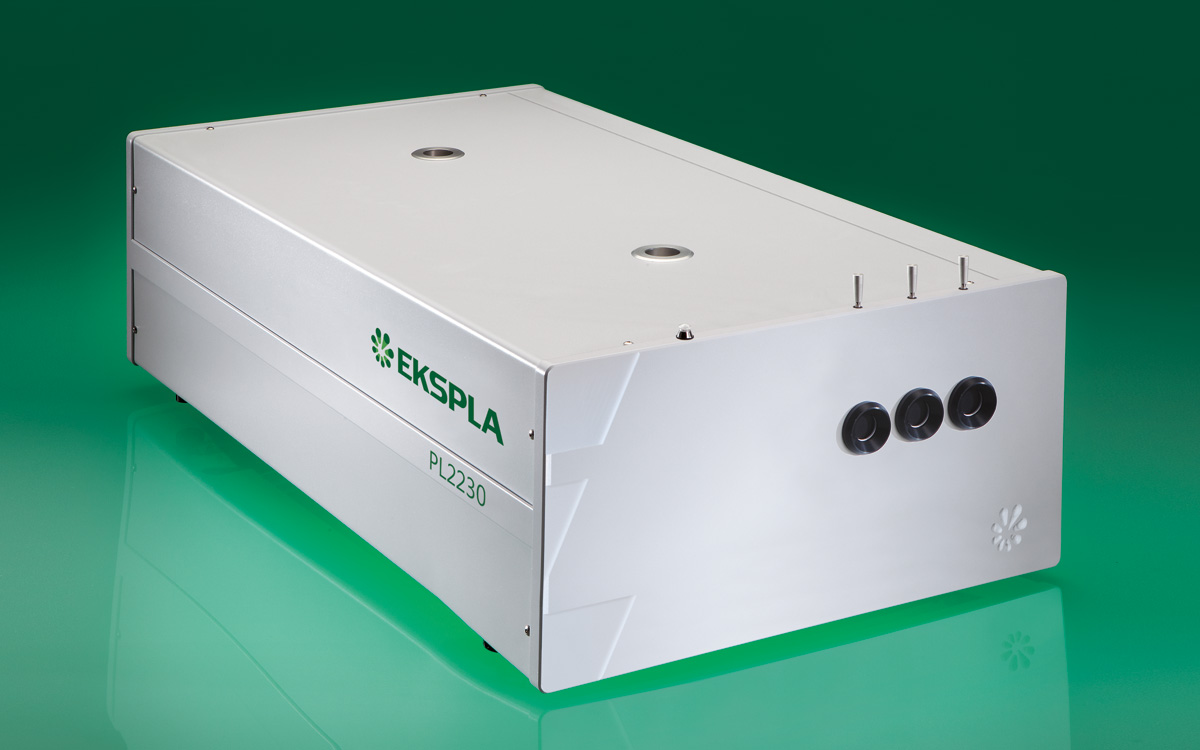
\includegraphics[width=\textwidth]{laser}
			\caption{Laser \emph{EKSPLA PL2231-50}.
% 				Převzato z~\autocite{ekspla-specs}.}
				Převzato z~\texttt{ekspla.com}.}
		\end{figure}
	\end{column}
	\end{columns}
\end{frame}

\section[E-FISH]{Electric field induced second harmonic generation}

\begin{frame}
	\frametitle{E-FISH}
	\begin{itemize}
		\item \emph{generování druhé harmonické frekvence v~elektrickém poli}
		\item opticky nelineární prostředí nebo vysoká intenzita
		\item dva fotony o~stejné frekvenci vytvoří nový
			o~dvojnásobné frekvenci
		\item $\efish \sim (I_\mathrm{laser} \elfield)^2$
	\end{itemize}
\end{frame}

\begin{frame}
	\frametitle{Kalibrace}
	\sisetup{per-mode=symbol}
	\graphicspath{{../efish/}}
	\input{../efish/plots/calib}
\end{frame}

\begin{frame}
	\frametitle{Elektrické pole výboje}
	\begin{figure}
		\centering
		\small
		\sisetup{per-mode=symbol}
		\graphicspath{{../efish/}}
		\input{../efish/plots/period-elfield}
		\caption{Časový vývoj intenzity elektrického pole
			v~různých místech výboje.}
	\end{figure}
\end{frame}

\section[TALIF]{Two-photon absorption laser-induced fluorescence}

\begin{frame}
	\frametitle{Dvoufotonová absorpce}
	\begin{columns}[c]
	\begin{column}{0.5\textwidth}
		\begin{itemize}
			\item nelineární optický jev
			\item absorpce dvou fotonů téže vlnové délky
		\end{itemize}
	\end{column}
	\begin{column}{0.5\textwidth}
		\begin{figure}
			\centering
			\begin{tikzpicture}[scale=0.5]
				\small
				\kryptontalifgrotrian
			\end{tikzpicture}
			\caption{Schéma dvoufotonové absorpce v~kryptonu.}
		\end{figure}
	\end{column}
	\end{columns}
\end{frame}

\end{document}
